\chapter[Convergence Module for Spoken Dialogue Systems]{Convergence Module for\\Spoken Dialogue Systems}
\label{chap:convergence_module_for_sdss}

\lettrine{T}{his} chapter introduces a computational model for measuring and applying phonetic convergence as well as a plug-and-use \acs{sds} module that integrates this model.

\pagebreak

\section{Modularization}
\label{sec:modularization}

%\begin{figure}[t]
%	\centering
%	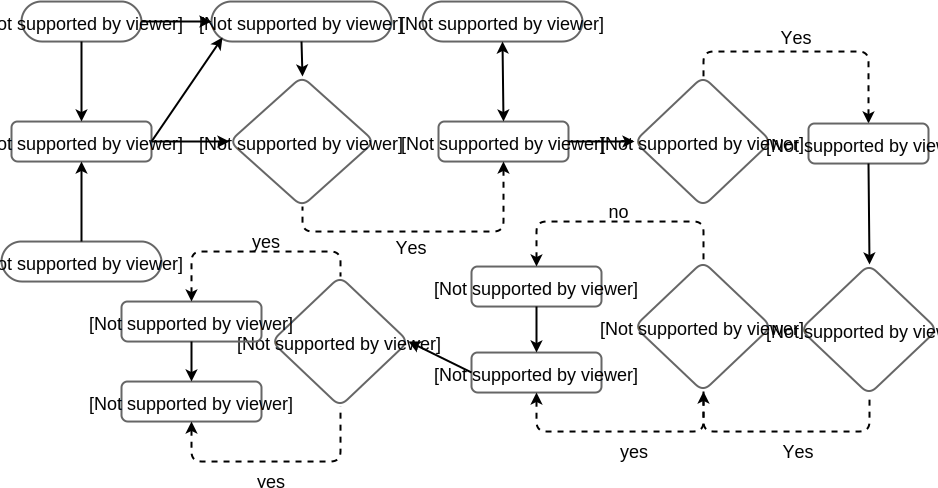
\includegraphics[width=\linewidth]{adaptation_module_pipeline}
%	\caption[Adaptataion pipeline for convergence module] {
%		Overview of the phonetic convergence pipeline used in the computational model. Rectangles
%		represent steps where an action is performed, round rectangles are inputs (either for external resources
%		or from the system), and diamonds stand for decision points. When a decision node does not have a “no”
%		outcome it means that the process is terminated (and therefore no convergence occurs) if the condition
%		is not met. The pipeline can only be successfully completed at the “Set feature’s new value” node.
%		However, if the “Add exemplar” action was performed prior to termination, the exemplar is not removed
%		and will be taken into consideration the next time the pipeline is triggered for the feature with which it is
%		associated. The “Feature definitions” come from the configuration file and can be changed by the user.
%	}
%	\label{fig:adaptation_module_pipeline}
%\end{figure}
\todo{here make an algorithm version of the pipeline (the figure comes later)}

\subsection{Computational model}
\label{subsec:computational_model}



\todo[inline]{some intro}

\subsubsection{Detecting segment exemplars}
\label{subsubsec:detecting segment exemplars}

The first step in the model is detecting segment in the user's utterance that can be ascribed to phonetic features the model aims to converge to.
This is done using CMU Sphinx\footnote{\url{https://cmusphinx.github.io/}} with some added functionality for omitting phoneme-level segments.
These features are defined, among other things, in a configuration file that is loaded by the model.
Each feature is represented by a YAML\footnote{YAML Ain't Markup Language \url{http://yaml.org/}} dictionary entry, which in turn contains a dictionary itself, where each key-value pair refer to a property of that feature.
For example, the entry

\begin{Verbatim}[tabsize=4, commandchars=\\\{\}]
- \textbf{`@\_length'}:
\textbf{phoneme}: AX
\textbf{context}: '.+ AX N'
\textbf{initial}: 0
\textbf{minimum}: 0
\textbf{maximum}: 80
\textbf{measure}: duration
\textbf{calculation}: decaying average
\textbf{sensitivity}: 0.5
\end{Verbatim}
\noindent
represents the feature \textit{@\_length} (length of a segment containing the phoneme schwa (\textipa{@})), which is indicated by \textit{AX} (value of the \textbf{phoneme} key) in the German CMU phoneme set.\todo{make sure this is really the phoneme set the system uses}
The value of the key \textbf{measure} is duration, which means that this feature is measure by the segment's length, as its name suggests.
Further more, the initial value in the model for this feature is 0 (\si{\milli\second}).
More properties will be explained in the subsections below.
This step is performed for each feature separately against each recognized phoneme (see \cref{alg:comp_model}).
Phonemes not ascribed to any defined feature are ignore.

\subsubsection{Filtering exemplars}
\label{subsubsec:filtering_exemplars}

Seeing that the target features are detected merely based on a phoneme, in which they might occur, additional filtering is required to retain only those instances where is does.
For example, the target feature \textit{@\_length} introduced in \cref{subsubsec:detecting segment exemplars} aims to capture the German phonological process of elision or epenthesis of \textipa{@} in word-final \textit{-en}\todo{put angle brackets around this}, as described by the rule described in \cref{eq:schwa_elision_rule}.
%(simplified version adapted from \citet[pp.\,142--143]{Benware1986phonetics}):
%
%\begin{equation}
%	\label{eq:schwa_elision_rule}
%	\text{\textipa{@}}\longrightarrow \varnothing \diagup
%	\left[\text{-son}\right] \ \_\_ \ \{\text{\#}, \left[\text{+const}\right]\}.
%	\todo{this rule is already defined in \cref{eq:}}
%\end{equation}
%\eqname{Phonological rule: schwa elision}

This filtering step comes to add any linguistic considerations related to the phonetic feature beside the phoneme itself.
Such considerations can phonemic context (defined as a phoneme regular expression in the \textbf{context} property) or range of acceptable values (defined by the \textbf{minimum} and \textbf{maximum} properties).
In the case of \textit{@\_length}, the phonemic context corresponds to a (simplified) context of the phonological rule described in \cref{eq:schwa_elision_rule}, and the value range defines the minimum and maximum length of the segment.
The range's goal is to filter out segments with unrealistic values (extremely long segment, unreliable formant values, etc.).
Any linguistic knowledge about the feature should be reflected in this step.
This important to make sure that all exemplars taken into account when calculating a new value for the feature (see \cref{subsubsec:calculating_changed_value} are sensible, to prevent unstable behavior of the model due to lack of linguistic knowledge or \ac{asr} and signal processing errors.

\subsubsection{Collecting exemplars}
\label{subsubsec:collecting_exemplars}

\todo{since in the ``theoretical'' part in Part 2 we say that this somehow represents both long and short term memories, explain that here we only deal with short memory explicitly, and long term memory is implicitly expressed by the starting value of the feature, i.e., the general (neutral) production of a speaker when no external influence is present,}

The remaining exemplars after filtering are stored and can be represented by a matrix $\mathcal{F}$, which contains the values of these exemplars.
As mentioned above, the exemplars are detected based on definition of each feature separately, and therefore each matrix $\mathcal{F}$ contains exemplars of a single feature.
Each exemplar is a row and each column is a dimension of this feature (e.g., a formant in a \textit{vowel quality} feature):

\begin{equation}
\label{eq:feature_matrix}
\mathcal{F} =
\begin{bmatrix} 
v_{11} & v_{12} & \dots  & v_{1m}\\
v_{21} & v_{22} & \dots  & v_{2m} \\
\vdots & \vdots & \ddots & \vdots \\
v_{n1} & v_{n2} & \dots  & v_{nm} 
\end{bmatrix}
\end{equation}
\eqname{A matrix of a phonetic feature}

\noindent
For example, the value $v_{21}$ is the first dimension of the second exemplar of the feature.
The model also defines a \textit{pool size}, which determines how many exemplars are kept for each feature.
This parameter aims to represent short-term mental memory of a feature's pronunciation.
That is, people are more likely to converge to utterances they heard recently than to something they heard before.\todo{can we say such a ``factual'' sentence without any reference/explanation?}
When a new exemplar is intercepted (after filtering), it is added to the pool (memory).
When a feature's pool is full (i.e., it reached its maximal size), the oldest exemplar is removed (forgotten) to make space for the newest one.
the exemplars in the pool are later used for calculating the system's change (\cref{subsubsec:calculating_changed_value}).
To calculate the change for each dimension (or sub-value) of a feature (like each formant of a vowel), the feature matrix is first transposed:

\begin{equation}
\label{eq:transposed_feature_matrix}
\textbf{$\mathcal{F}$}^\top =
\begin{bmatrix} 
v_{11} & v_{21} & \dots  & v_{n1}\\
v_{12} & v_{22} & \dots  & v_{n2} \\
\vdots & \vdots & \ddots & \vdots \\
v_{1m} & v_{2m} & \dots  & v_{nm} 
\end{bmatrix}
\end{equation}
\noindent
In this matrix, each row refers to a single dimension of the feature.
For example, the second row contains the value of the second dimension of each exemplar.

\subsubsection{Calculating a new value}
\label{subsubsec:calculating_changed_value}

The new value of a feature is calculated based on its exemplar pool (\cref{eq:transposed_feature_matrix}).
The relation between these values and the new value the system will use for this feature is a key aspect of the whole process.
A \textit{calculation method} is needed to define this relation ship.
Different calculation methods can represent different types of relations and approaches.
We define a function $g$ that maps a vector to a scalar (one feature dimension) and a function $\mathcal{G}$ which maps a matrix to a vector (the entire feature) by applying $g$ to all the row vectors in $\mathcal{F}$, both based on a user-defined calculation method:

\begin{equation}
	\label{eq:matrix2vec}
	g: \mathbb{Q}^{m} \longrightarrow \mathbb{Q}, \qquad \mathcal{G}: \mathbb{Q}^{n \times m} \longrightarrow \mathbb{Q}^{m} 
\end{equation}

\textit{Decaying average} was used as a baseline method.
This measure is similar to normal average, only that in this variation each value contributes exponentially less to the overall average, so that the last (newest) value contributes the most.
Adding such property to the measure gives more weight to new exemplars that were received chronologically closer to present time, and less weight to older exemplars that stayed longer in memory (and had more weight when they were new).
Using this measure comes to support the analogy of the exemplar pool to short-term memory, which remembers recent event better than oder ones.
Decaying average is a recursive measure described by
\begin{equation}
\label{eq:decaying_average}
\mu_n = \frac{1}{n}\sum_{i = 2}^{n}(\eta v_i + (1 - \eta )\mu_{i-1}),
\end{equation}
\eqname{Decaying average}
%
with $n$ being the number of elements in a row of the transposed feature matrix (\cref{eq:transposed_feature_matrix}), $\eta$ the decay rate, $\mu_{i-1}$ the decaying average of the previous element, and $v_i$ the value of the $i$-th element.
However, every function that can map vectors to scalars can be used here to experiment with different methods.

Before setting the updated value as the feature's value (see \cref{subsubsec:setting_the_new_value}), the balance between the feature's current value and its calculated pool value needs to be set.
This is defined by the \textbf{sensitivity} property (or \textit{convergence rate}).
The purpose of this parameter is to model the speaker's sensitivity to changes (hence the properties name), and it is used as follows:

\begin{equation}
\Upsilon \equiv \mathcal{C}_u = \rho \upsilon + \left(1 - \rho \right) \mathcal{C}_{u-1} 
\label{eq:convergence_rate}
\end{equation}
\noindent
where $\Upsilon$ is the new feature value (i.e., the value after update $u$), $\upsilon$ is the calculated pool after applying $\mathcal{G}$, $\mathcal{C}_{u-1}$ is the current value of the feature (after the previous update), and $\rho$ is the convergence rate.
A $\rho$ value of 0 means that no convergence occurs (the current value is retained), a value of 1 will result in complete convergence (the current value is ignored), and $\rho=0.5$ will result in an average between the two.
While the convergence rate is typically a value between 0 and 1, smaller and greater values could be meaningful in some applications to achieve divergence or over-convergence, respectively.

Having found in previous work that people's convergence in both \ac{hhi} and \ac{hci} varies considerably \citep{Gessinger2017Interspeech}, this parameter needs to be tuned with respect to the other parameters to obtain convergence steps that are comparable to natural speech convergence.
It can be use to achieve certain behaviors during the interaction.
For instance, in a tutoring system for pronunciation training, the desired behavior might be for the system to diverge from users' input when it detects that their pronunciation is wrong.
By reflecting the users' utterance with diverged pronunciation (instead of explicitly pointing out their mistake), the user receives auditory feedback in a more \enquote{conversational} learning process.

%\begin{equation}
%	\lambda\mathcal{M} = \lambda
%	\begin{pmatrix} 
%		v_{11} & v_{12} & \dots  & v_{n}\\
%		v_{21} & v_{22} & \dots  & v_{2n} \\
%		\vdots & \vdots & \ddots & \vdots \\
%		v_{e1} & v_{e2} & \dots  & v_{en} 
%	\end{pmatrix}
%\end{equation}
%
%\begin{equation}
%	\mathcal{M}_i' = g(\mathcal{M}^{\intercal}_{i \leq m})
%	\label{eq:value_calculation}
%\end{equation}
%\noindent
%where $\mathcal{M}^{\intercal} \in \mathbb{Q}^{m \times n}$ is the transposed exemplar matrix (which comprises vectors of dimension values instead of vectors of exemplar values), $g$ is the chosen calculation method to apply to each vector, $\mathcal{M}' \in \mathbb{Q}^{m \times n}$ is the matrix with the pool values for each dimension of the feature, $i$ is the vector index, and $m$ is the number of rows in $\mathcal{M}^{\intercal}$.

%$\lVert P \rVert $ refers to the Euclidean Norm (or vector's magnitude).

\subsubsection{Setting the new value}
\label{subsubsec:setting_the_new_value}
\todo[inline]{mention also that we limit the final value to prevent imitation}

The final step is to set the newly calculated value (\cref{subsubsec:calculating_changed_value} as the new value for the feature in the model.
After this step ,this new value will be used whenever this feature is used by a system using this model (more details in \cref{subsec:computational_model}).
Although this step is fairly straight forward, there is still an important issue to take into consideration here, namely \textit{user imitation}.
After some turns (or with a certain combination of parameter values), it might happen that the model calculated a value very close to the user's input.
To avoid imitation, the new value is limited in how close it is allowed to get to the exemplars.
This is done by the global property \textbf{ConvergenceThreshold}, which defines the maximally allowed proximity (in percentage) the new value is allowed to have:
Setting this property to 0.8 (\SI{80}{\percent} means that the new value is not allowed to be changed more than (\SI{80}{\percent} of the difference between the current value and the pool's value (and be set to (\SI{80}{\percent} in case it exceeded this threshold).
Of course, the limitation can also be set to 1 to allow the new value be as similar as \SI{100}{\percent} to the pool's value -- i.e., not limiting it.
The maximal value allowed by the limitation is defined by

\begin{equation}
\label{eq:conv_limit}
\Lambda = \delta \upsilon \left(1 - \lambda \right),
\end{equation}
\noindent
where $\Lambda$ is the maximum convergence value allowed, $\delta$ is set to 1 if the converging values are increasing or $-1$ in case they are decreasing (see \cref{eq:direction}), and $\lambda$ is the convergence limit parameter ($\lambda=0.8$ in the example above).
\noindent
Note that the actual value of this limit depends on the direction in which the convergence occurs, which is defined by

\begin{equation}
\label{eq:direction}
\delta = 		
\begin{cases}
\ \ \ 1 & \text{if } \upsilon \geq \mathcal{C}_t\\
-1 & \text{otherwise}
\end{cases}.
\end{equation}
\eqname{Determining accommodation direction}
\noindent
That is, if the converging values are increasing, the limit's value will be smaller than the pool value;
and if the values are decreasing toward the pool value, the limit's value will be greater than the pool value.
Ultimately, the final updated value for the feature is determined as follows:

\begin{equation}
\label{eq:new_value}
\Upsilon = 		
\begin{cases}
% newValue - (newValue - (newValue * convergenceThreshold)) * direction
\upsilon - \Lambda & \text{if }\upsilon - \Upsilon \leq \delta\Lambda\\
\Upsilon \text{ (unchanged)} & \text{otherwise}
\end{cases}.
\end{equation}
\eqname{Setting accommodation limit}
\noindent
It is important to mention that this limitation not only comes to prevent situations where the model mimics and user's behavior (which might lead to intimidation), but is also loyal to behaviors observed in the experiment, where participants only converged up to a certain limit, hence the name of this property.

The entire computational model is described in \cref{alg:comp_model}.
Further details about the model and all the steps can be found in \citet{Raveh2017Interspeech}.

\addtocounter{myequations}{1}
\begin{algorithm}[t]
	\caption{Phonetic responsiveness}
	\label{alg:comp_model}
	\eqname{Phonetic responsiveness algorithm}
	\algorithmcaption{Note that \emph{ASRInput} (\cref{line:asrinput}) must not only contain the $n$-best hypotheses, but also their phoneme lists (in chronological order).
	For improving performance, using a single hypothesis is recommended for a small language model and/or when very short sentences are expected.
	Since only the target phonemes are treated (and suprasegmental features where the specific phonemes do not matter), it might not be crucial to get a completely correct \ac{asr} hypothesis if not required for continuing the interaction.
	For example, a \ac{capt} system might rely solely on the realization of specific phonemes, regardless of what the user said or should have said.}
	\DontPrintSemicolon
	\SetKwInOut{Input}{Inputs}
	\SetKwInOut{Output}{Output}
	
	\Input{\underline{$ASRInput$} -- recognized user speech\newline
		   \underline{$targetPhonemes$} -- convergence features\newline}
	\Output{list of feature vectors with converged values\newline}
	
	\ForEach {(phoneme $\in$ ASRInput) $\in$ targetPhonemes}{ \label{line:asrinput}
		$feature \gets$ $phoneme$.associatedFeature\;
		$context \gets feature$.phoneticContext\;
		\uIf {\textbf{not} matches(phoneme, context)}{ \tcp*{filter based on context}
			break\;}
		\uIf {inRange($phoneme$, $allowedRange$)}{ \tcp*{filter based on value range}
			\uIf {poolSize=maxPoolSize}{
				deleteOldestExemplar()\;}
			feature.addExemplar($phoneme$)\;}
		\uElse{
			break\;}
		\uIf {toUpdate $=0$}{
			$method \gets feature$.calculationMethod\;
			$poolValue \gets method$.calculate(pool)\;
			$newValue \gets rate\cdot poolValue + (1-rate)\cdot feature.$value\;
			$threshold \gets convergenceLimit \cdot poolValue$\;
			\uIf {$newValue > threshold$}{ \tcp*{limit convergence}
				$newValue \gets threshold$\;}
			$feature$.value $\gets newValue$\;
			{\em toUpdate $\gets$ updatefrequency}\;}
		\uElse{
			{\em toUpdate $\gets$ toUpdate - 1}\;}}
\end{algorithm}
\todo[inline]{make algorithm more readable, change, variable/method names, etc.}

\section{Integration}
\label{sec:integration}

\begin{figure}[t]
	\centering
	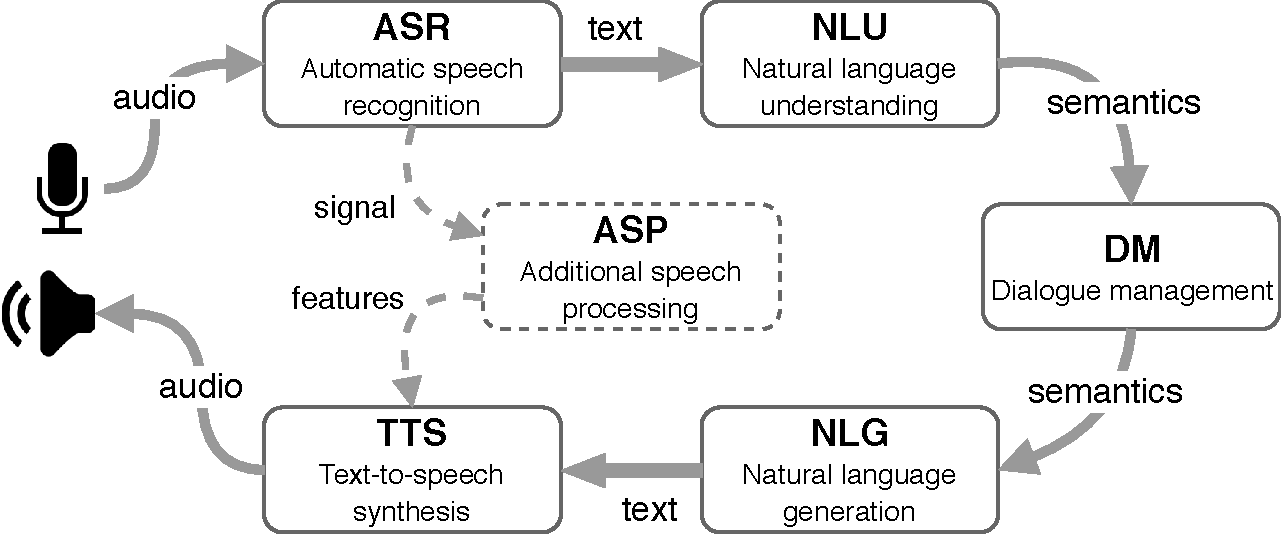
\includegraphics[width=\linewidth]{sds_architecture_ext}
	\caption[Proposed extended architecture of a spoken dialogue system] {
		Suggested architecture for a spoken dialogue system with the phonetic convergence module (conf.\ \cref{fig:sds_architecture}).
		The module connects the \ac{asr} and the \ac{tts} modules, and performs additional speech processing used phonetic for adaptation, like feature detection and extraction.
	}
	\label{fig:adaptation_module_architecture}
\end{figure}
